\documentclass[Main.tex]{subfiles}
\begin{document}
\section{Introduction}
Over the past two decades the field of swarm intelligence has evolved from intertwined branches of mathematics, physics, biology, traditional robotics, and artificial intelligence; attempting to apply observations of physical and biological systems to artificial ones. This has led to novel approaches in the design and analysis of multi-agent systems and the algorithms associated with them. It has spawned an entirely new field of research called \emph{swarm robotics}. A definition of swarm robotics as given by \c{S}ahin and Spears is,
\begin{quote}\emph{The study of how a swarm of relatively simple physically embodied agents can be constructed to collectively accomplish tasks that are beyond the capabilities of a single one.}\cite{Sahin2005}
\end{quote}

This literature survey paper attempts to collate the research done so far in this relatively new field, while focusing on mathematical and computational modeling techniques that have been developed to help describe the temporal and spatial evolution of a swarm of robots programmed to perform specific, collaborative tasks. While literature reviews for swarm robotics models already exist\cite{Winfield2005, Lerman2005}, this paper attempts to include both, non-spatial and spatial modeling techniques as well as discussions on parameter discovery and optimization which is an area I am particularly interested in.

Swarm systems have many benefits over traditional, centralized robot systems. The robots used in swarm applications are generally many orders of magnitude smaller (centimeters vs. meters, grams vs. kilograms) and simpler in design ($<10$ actuators vs. $100$s of actuators) than conventional robots. Also, most swarm systems are homogeneous---robots with identical software/hardware are used to complete the assigned task. This makes swarm systems easily scalable while simultaneously keeping manufacturing and maintenance costs of the hardware low. Though, perhaps their greatest advantage is system stability and robustness to error. Many well known swarm algorithms such as Ant Colony Optimization, Virtual Pheromone Tracking~\cite{Payton2005}, and Particle Swarm Optimization  rely on the fact that most agents (ants/particles) are on a non-optimum trajectory so as to maximize coverage over the search space. This concept also carries over to a hardware swarm system. Most swarm systems consist of small, relatively simple robots that are only capable of limited and noisy sensing, communication and actuation. This means that while no single robot alone is capable of performing the task assigned, the system as a whole is resilient to individual errors from agents and is capable of completing the task.

\begin{figure}[!ht]
\centering\begin{subfigure}{.5\textwidth}
\centering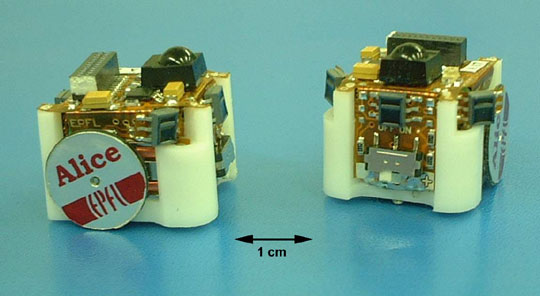
\includegraphics[height=4cm,width=6.5cm]{alicerobot.png}
\caption{Alice robot}
\end{subfigure}~
\centering\begin{subfigure}{.5\textwidth}
\centering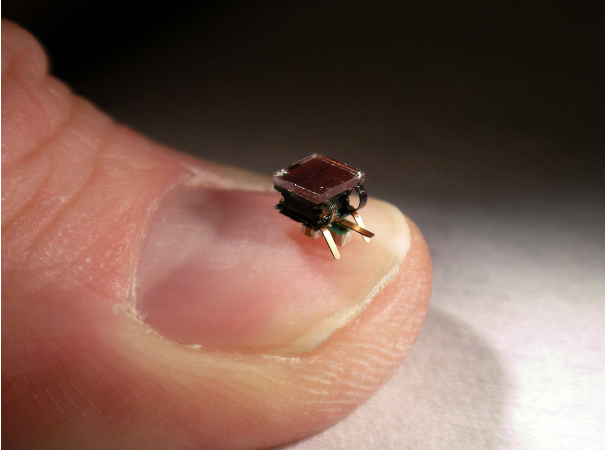
\includegraphics[height=4cm,width=6.5cm]{iswarm.png}
\caption{I-SWARM robot concept}
\end{subfigure}\vspace{1cm}
\centering\begin{subfigure}{.5\textwidth}
\centering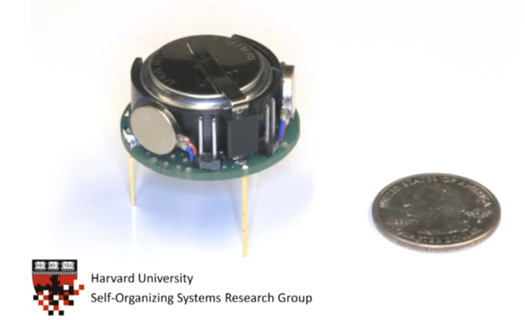
\includegraphics[height=4cm,width=6.5cm]{kilobotrobot.png}
\caption{Kilobot robot}
\end{subfigure}~
\centering\begin{subfigure}{.5\textwidth}
\centering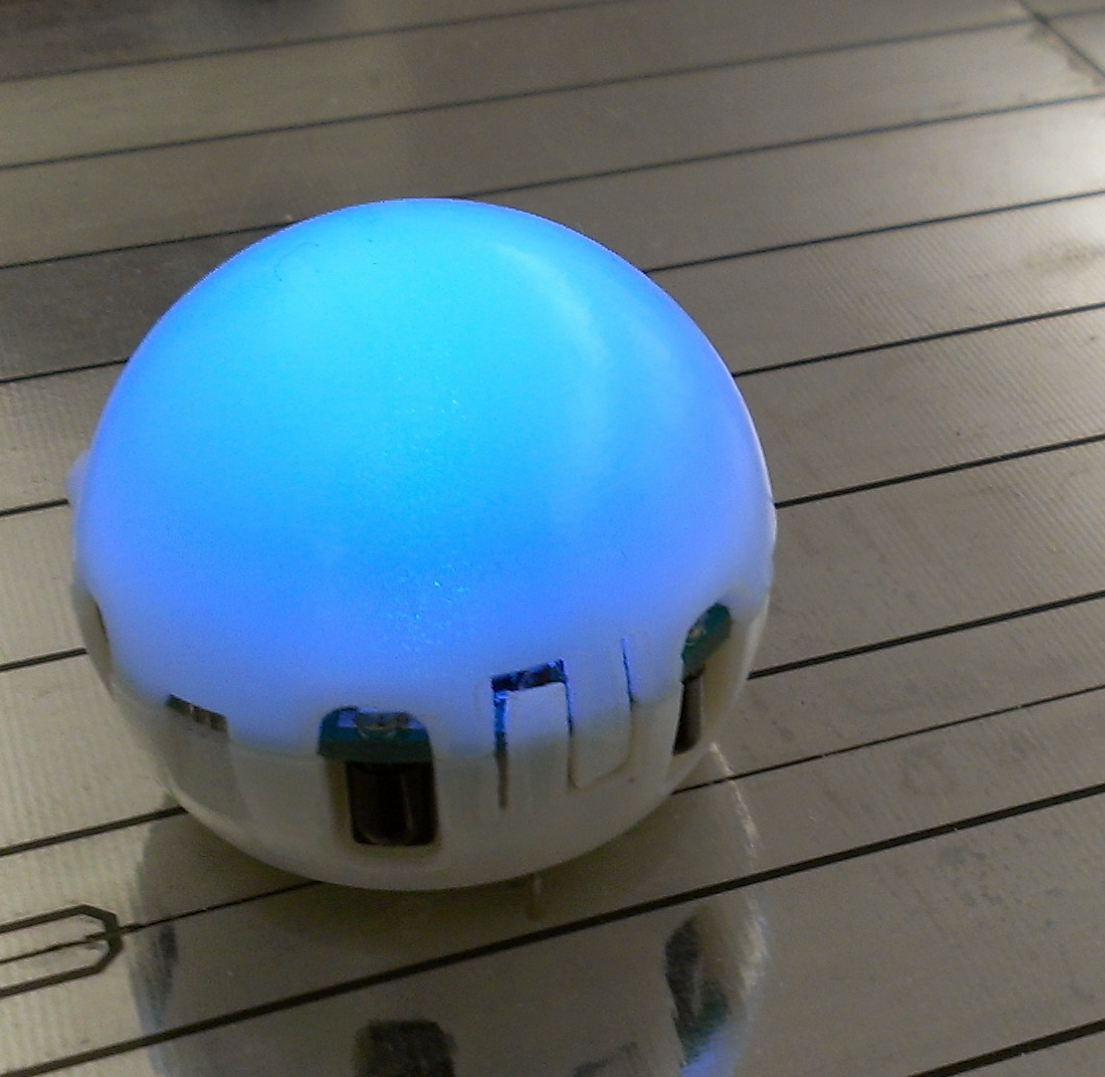
\includegraphics[height=4cm,width=5cm]{dropletrobot.png}
\caption{Droplet robot}
\end{subfigure}
\caption{}\label{fig:swarmbots}
\end{figure}

So then, why do we want to model swarm systems? While much progress has been made in the development and production of miniature swarm robots such as, Alice, Khepera, Kilobots, etc.\cite{Dorigo2005, Seyfried2005, Mondada2009, Caprari1998, Rubenstein2012} there is still no viable large scale ($> 10,000$ units) implementation available. It is also difficult to observe and measure large scale system properties during physical experiments without the use of more sophisticated tools like machine vision and global communication. Thus, many algorithms in the field have been developed and formally proven using mathematical models and computer simulation, generally backed up by small scale physical experiments. While physics based simulators such as Webots\cite{Michel1998} are indeed helpful for rapid experimentation and observation, they take time to develop and are computationally intensive processes. Simulations are generally faster than physical experiments but slower than mathematical models. They are also not exact---by their very nature---and therefore could miss emergent behavior or other macroscopic properties as they tend to simulate systems on the individual agent or microscopic level. 

Methods for modeling a swarm system are therefore extremely important as they provide a formal understanding of the relationship between control parameters, physical properties, and performance. These models can then be used to provide formal guarantees on performance as well as system identification and parameter optimization\cite{Correll2006a, Correll2008}.

With this motivation for modeling swarm systems in mind, the rest of the paper is structured as follows. The next section describes and defines the technical terms that will be used for the remainder of this paper. While many of the terms, such as, spatial, non-spatial, robot, etc. can have very broad and general definitions, the section aims to define them more specifically in the context of this survey paper and it's purpose; to explain the different modeling and optimization techniques in use for studying swarm robotics algorithms. Section 3 outlines a general methodology often used in the swarm robotics community for designing and optimizing a robot controllers and developing swarm system models. Section 4 covers non-spatial modeling applications using an array of well known swarm robot experiments. The end of this section also describes my original work done in designing a novel robot controller for multi-robot collaboration based on a sigmoid threshold response function. In the next section we begin to explore the less understood realm of spatial models in swarm robotics. The models discussed in this section are heavily inspired by physical models of Brownian motion and involve the use of the Langevin equation and the Fokker--Planck equation (also known as the Kolmogorov forward equation). Finally, the conclusion provides a short summary of open questions in the field of swarm system modeling and areas of research I am interested in pursuing further.

\end{document} 